%        File: area.tex
%     Created: Tue Mar 15 11:00 AM 2016 E
% Last Change: Tue Mar 15 11:00 AM 2016 E
%
\documentclass{standalone}
\usepackage{tikz}
\usepgflibrary{arrows.meta}
\usetikzlibrary{calc}
\pgfdeclarelayer{background}
\pgfsetlayers{background,main}
\begin{document}
\small
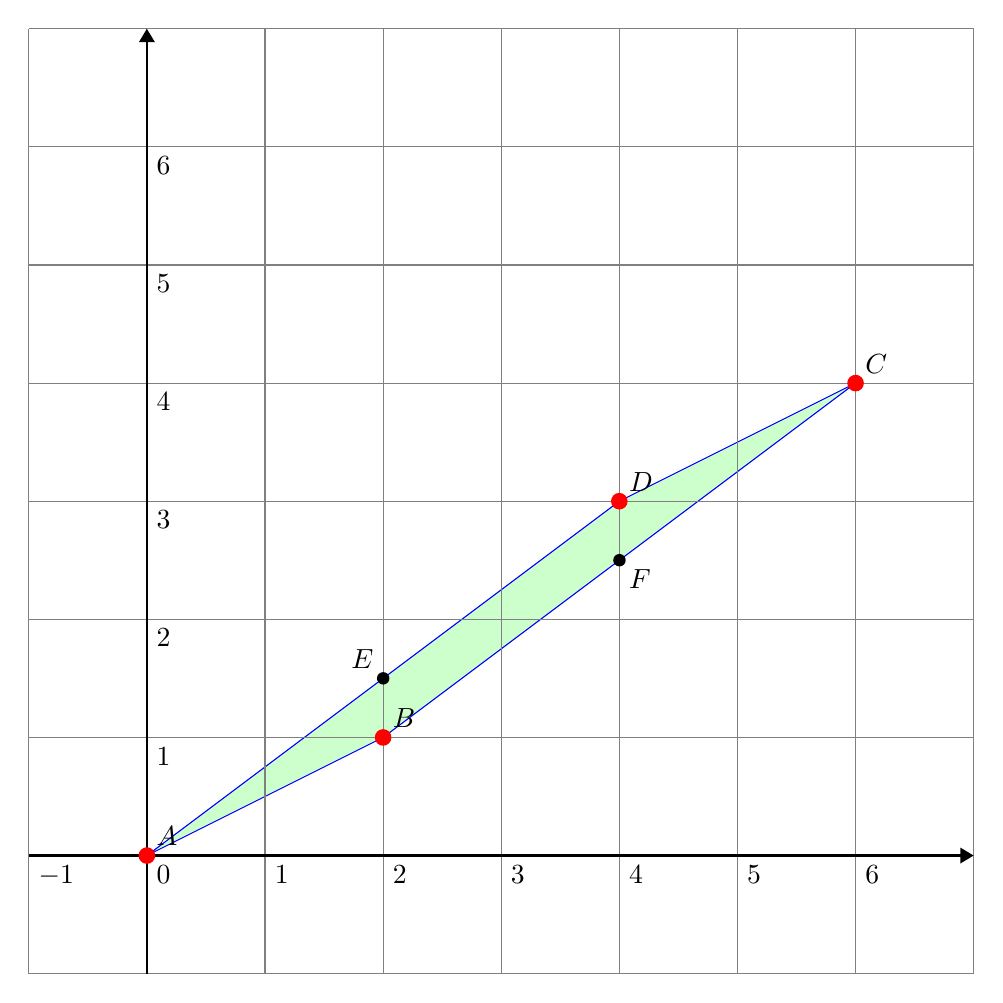
\begin{tikzpicture}[scale=1.5]
    \draw[thin, gray] (-1,-1) grid (7,7);
    \draw[thick,-{Triangle[]}] (-1,0) -- (7,0);
    \draw[thick,-{Triangle[]}] (0,-1) -- (0,7);
    \foreach \i in {-1,0,...,6}{
    \node[below right] at (\i,0) {$\i$};
    }
    \foreach \i in {1,...,6}{
    \node[below right] at (0,\i) {$\i$};
    }
    \foreach \pt/\lab in {(0,0)/A, (2,1)/B, (6,4)/C, (4,3)/D}{
    \fill[red] \pt circle[radius=2pt] coordinate (\lab);
    \node[above right] at \pt {$\lab$};
    }
    \begin{pgfonlayer}{background}
        \draw[blue,fill=green!20!white] (A)
        \foreach \pt in {B, C, D, A}{
         -- (\pt)};
    \end{pgfonlayer}
    \coordinate (E) at ($ (A)!.5!(D) $);
    \coordinate (F) at ($ (B)!.5!(C) $);
    \fill[black] (E) circle[radius=1.5pt];
    \node[above left] at (E) {$E$};
    \fill[black] (F) circle[radius=1.5pt];
    \node[below right] at (F) {$F$};
\end{tikzpicture}
\end{document}


